\documentclass[crop=false, class=book]{standalone}

\begin{document}
	\chapter{Introduzione}
	
	Il sequenziamento del DNA costituisce una tecnica fondamentale per lo studio del genoma di una specie, perché permette di determinare l'ordine dei nucleotidi che costituiscono il DNA. Tale processo trova applicazione in molti studi biologici che riguardano vari ambiti, come ad esempio la medicina riproduttiva, l'oncologia o l'infettivologia, attraverso indagini tra cellule diverse dello stesso individuo o lo studio delle mutazioni genetiche tra individui di una stessa specie \cite{shendure2012expanding}. 

	\section{Metodi di sequenziamento}
		
		\subsection{Metodi di prima generazione}
		Le prime tecniche di sequenziamento del genoma furono sviluppate nella seconda metà del Novecento. Nel 1977 infatti vennero pubblicati due metodi di sequenziamento: il metodo Sanger, nel quale la sequenza di nucleotidi viene frammentata grazie a un terminatore di catena \cite{sanger1977DNA,sanger1977nucleotide}, e il metodo di  Maxam e Gilbert, in cui vengono utilizzati reagenti chimici per tagliare il DNA in frammenti in corrispondenza di basi specifiche \cite{maxam1977new}. Entrambi i metodi prevedono la misurazione dei frammenti creati tramite elettroforesi su gel di poliacrilammide con una corsia per base, in modo che siano separati in ordine di lunghezza e sia possibile dedurre l'ordine delle basi della sequenza in esame \cite{shendure2017DNA}. Mentre il metodo Maxam-Gilbert è stato progressivamente accantonato per la difficoltà tecnica e l'uso di sostanze tossiche che lo caratterizzano, il metodo Sanger è stato affinato con l'utilizzo di marcatori fluorescenti diversi per ogni base, che un lettore laser può distinguere restituendo la sequenza di basi di ogni frammento.
		
		\subsection{Shotgun assembly}
		Il sequenziamento del genoma può essere fatto su sequenze più lunghe, come un intero cromosoma, tramite \textit{shotgun assembly}, metodo suggerito già nel 1979 \cite{staden1979strategy}. Il genoma iniziale viene duplicato in modo da produrne più copie identiche, le quali vengono tagliate in frammenti casuali (\textit{shotgun}) che possono essere letti singolarmente. Si procede quindi con l'\textit{assembly}, cioè la ricostruzione del genoma iniziale. L'assemblamento dei frammenti può avvenire con due metodi diversi, tramite \textit{reference assembly} o con \textit{de novo assembly}.
			\paragraph{Reference assembly}
			Per la ricostruzione del genoma viene utilizzata una sequenza di riferimento il più possibile simile alle letture disponibili, che permette di assemblare i frammenti più facilmente tramite allineamento \cite{wajid2014do}.
			
			\paragraph{De novo assembly}
			Se non è disponibile una sequenza di riferimento appropriata, i frammenti vengono legati insieme identificando pattern sovrapponibili e formando più \textit{contig}, che vengono poi combinati con altre tecniche algoritmiche \cite{noune2017dynamics}. 
		
		\paragraph{}
		Ogni frammento viene quindi allineato con gli altri shotgun disponibili, formando una sequenza comune, il \textit{consensus}; ciascuna base della sequenza assemblata ha una certa copertura (\textit{coverage}), che è pari al numero di letture che contribuiscono al posizionamento della base nel consensus. La figura~\vref{fig:assembly} mostra un semplice esempio di questo metodo.
		
		\begin{figure}[h]
			\centering
			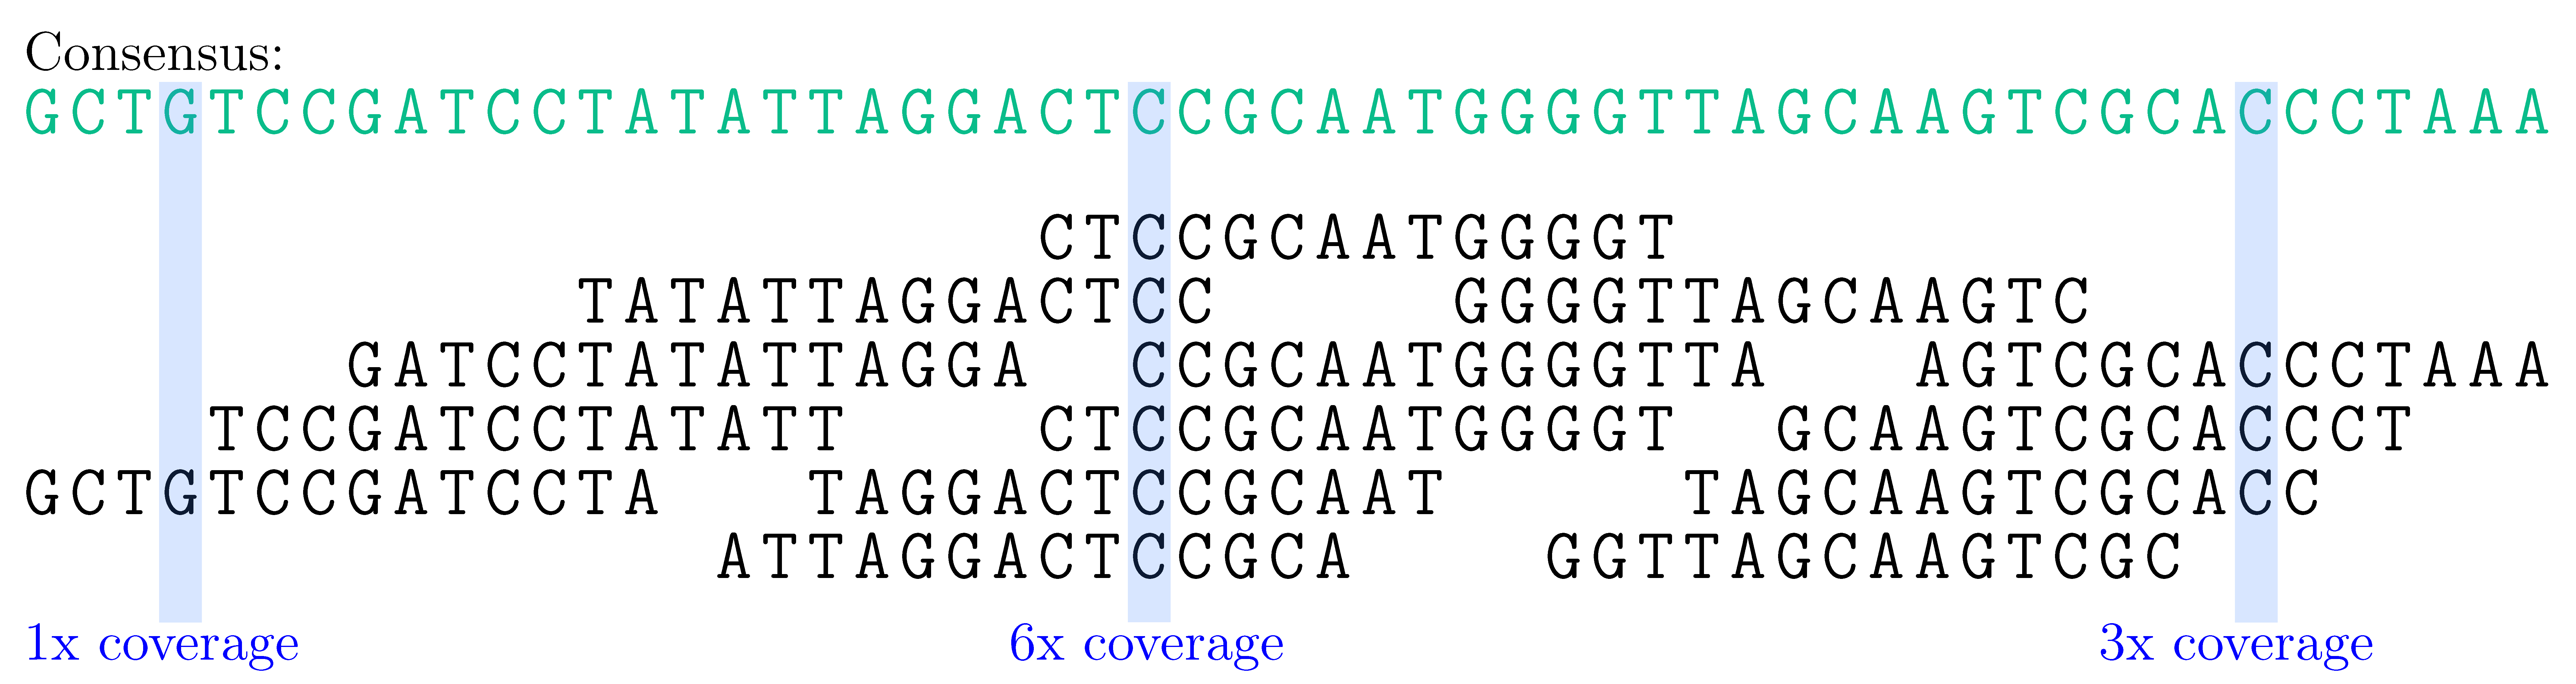
\includegraphics[width=\textwidth]{capitoli/introduzione/assembly.png}
			\caption{Esempio di allineamento di shotgun per la formazione del consensus.}
			\label{fig:assembly}
		\end{figure}
		
		\subsection{Metodi di seconda e terza generazione}
		I metodi di seconda generazione, comunemente chiamati \textit{NGS} - \textit{Next Generation Sequencing}, introducono un'elevata parallelizzazione del sequenziamento. Sostanzialmente, i vari metodi disponibili (come ad esempio \textit{454}, \textit{Illumina} o \textit{Ion Torrent}) prevedono inizialmente la frammentazione del genoma da sequenziare, e l'unione di particolari sequenze ai frammenti creati. Essi vengono quindi amplificati tramite \textit{emPCR} o \textit{bridge amplification} \cite{heather2016sequence}, e possono essere sequenziati con letture parallele, spesso facendo uso di molecole fluorescenti. Segue quindi l'assemblamento delle letture ottenute per la ricostruzione della sequenza originale.
		
		Il sequenziamento con metodi di terza generazione, quali \textit{Nanopore} o \textit{MinION}, si basano sul sequenziamento a singola molecola \cite{shendure2017DNA}. Pur mostrando un'efficienza maggiore rispetto ai metodi precedenti, sono attualmente ancora in fase di sviluppo.
		
	
	\section{Stima della dimensione del genoma}
	Il problema della misurazione della dimensione del genoma costituisce un argomento di interesse, perché oltre a fornire informazioni sulla sua evoluzione \cite{gregory2005synergy}, permette di approssimare la quantità di dati che verranno prodotti nel sequenziamento e di valutare la complessità delle sequenze assemblate \cite{sun2017findGSE}. 
	
	Di seguito sono elencate le due principali tipologie di metodi per la stima della dimensione del genoma, basate rispettivamente su approcci sperimentali o computazionali.
	
		\subsection{Metodi sperimentali}
		Inizialmente la ricerca scientifica ha cercato di stimare la dimensione del genoma con approcci biochimici, come ad esempio i metodi \textit{Feulgen photometry} o \textit{flow cytometry}. Tali metodologie però, oltre ad essere costose dal punto di vista economico e poco efficienti, devono basarsi su genomi specifici di riferimento \cite{pucker2019MGSE, sun2017findGSE}.

		\subsection{Metodi computazionali}
		Grazie all'aumento delle capacità computazionali, sono stati sviluppati metodi che possono calcolare la lunghezza del genoma utilizzando i dati ricavati dall'assemblaggio di shotgun. Dato che i dati assemblati sono di solito incompleti, è più conveniente cercarne di stimare la dimensione, utilizzando ad esempio i \textit{k-mer}. 
		
		In questa trattazione verranno analizzati e confrontati vari approcci algoritmici che utilizzando i k-mer compiono la stima della dimensione del gemoma.
	
	
	\section{Sequenze di lunghezza k: i k-mer}
	I \textit{k-mer} sono tutte le sottostringhe di lunghezza $k$ presenti nella sequenza del genoma \cite{marcais2011fast}. Si prenda ad esempio la sequenza descritta in~\vref{seq}. 
	\begin{equation}
	\label{seq}
		AGATTCGC 
	\end{equation}
	
	I k-mer di lunghezza $k=1$ saranno le quattro basi che formano la sequenza: $G, T, A, C$. Ponendo invece $k=2$, i k-mer trovati saranno tutte le coppie formate da due basi: $AG, GA, AT, TT, TC, CG, GC$. \\
	\noindent
	Allo stesso modo, per $k=3$ le sequenze sono: $AGA, GAT, ATT, TTC, TCG, CGC$.

	Il listing~\vref{lst:kmer-count} mostra una semplice implementazione in pseudocodice per determinare i k-mer di lunghezza \verb|k|, iterando la sequenza di input \verb|seq| e dando in output tutte le sottostringhe di lunghezza \verb|k| presenti in essa.
	
	\begin{center}
		\begin{minipage}{0.95\textwidth}
			\begin{lstlisting}[caption={Algoritmo in pseudocodice per la costruzione dei k-mer.}, label={lst:kmer-count}, language=pseudocode]
				procedure k-mers(seq, k)
					lunghezza = length(seq)
					arr = array di L - k + 1 stringhe vuote
						
					// La sequenza iniziale viene iterata, 
					// salvando il k-mer n-esimo nell'array di output
					for n = 0 to L - k + 1 escluso do 
						arr[n] = sottostringa di seq da seq[n] a seq[n+k] escluso
					
					return arr
			\end{lstlisting}
		\end{minipage}
	\end{center}
		
	Dato che il numero di k-mer aumenta esponenzialmente all'aumentare del parametro \verb|k|, sono necessari algoritmi più complessi per il calcolo dei k-mer, come ad esempio \textit{Jellyfish}~\cite{marcais2011fast} o \textit{KMC2}~\cite{deorowicz2015KMC}.
	
	\subsection{K-mer profile}
	\label{subsec:kmerprofile}
	Il \textit{k-mer profile}, detto anche \textit{k-mer spectrum}, rappresenta un indicatore della complessità del genoma preso in esame. Date in input le letture shotgun del genoma, esso mostra il numero di volte che ogni k-mer viene trovato rispetto la quantità di k-mer distinti presenti, ovvero la molteplicità di ciascun k-mer nella sequenza rispetto il numero di k-mer con quella molteplicità \cite{mapleson2017kat}. Un esempio di k-mer profile è mostrato dalla figura~\vref{fig:profilecomp} tratta da \cite{sohn2016present}, in cui si può notare come la natura del genoma influenzi direttamente il grafico in ogni sua componente. 

	
	\begin{figure}[h]
		\centering
		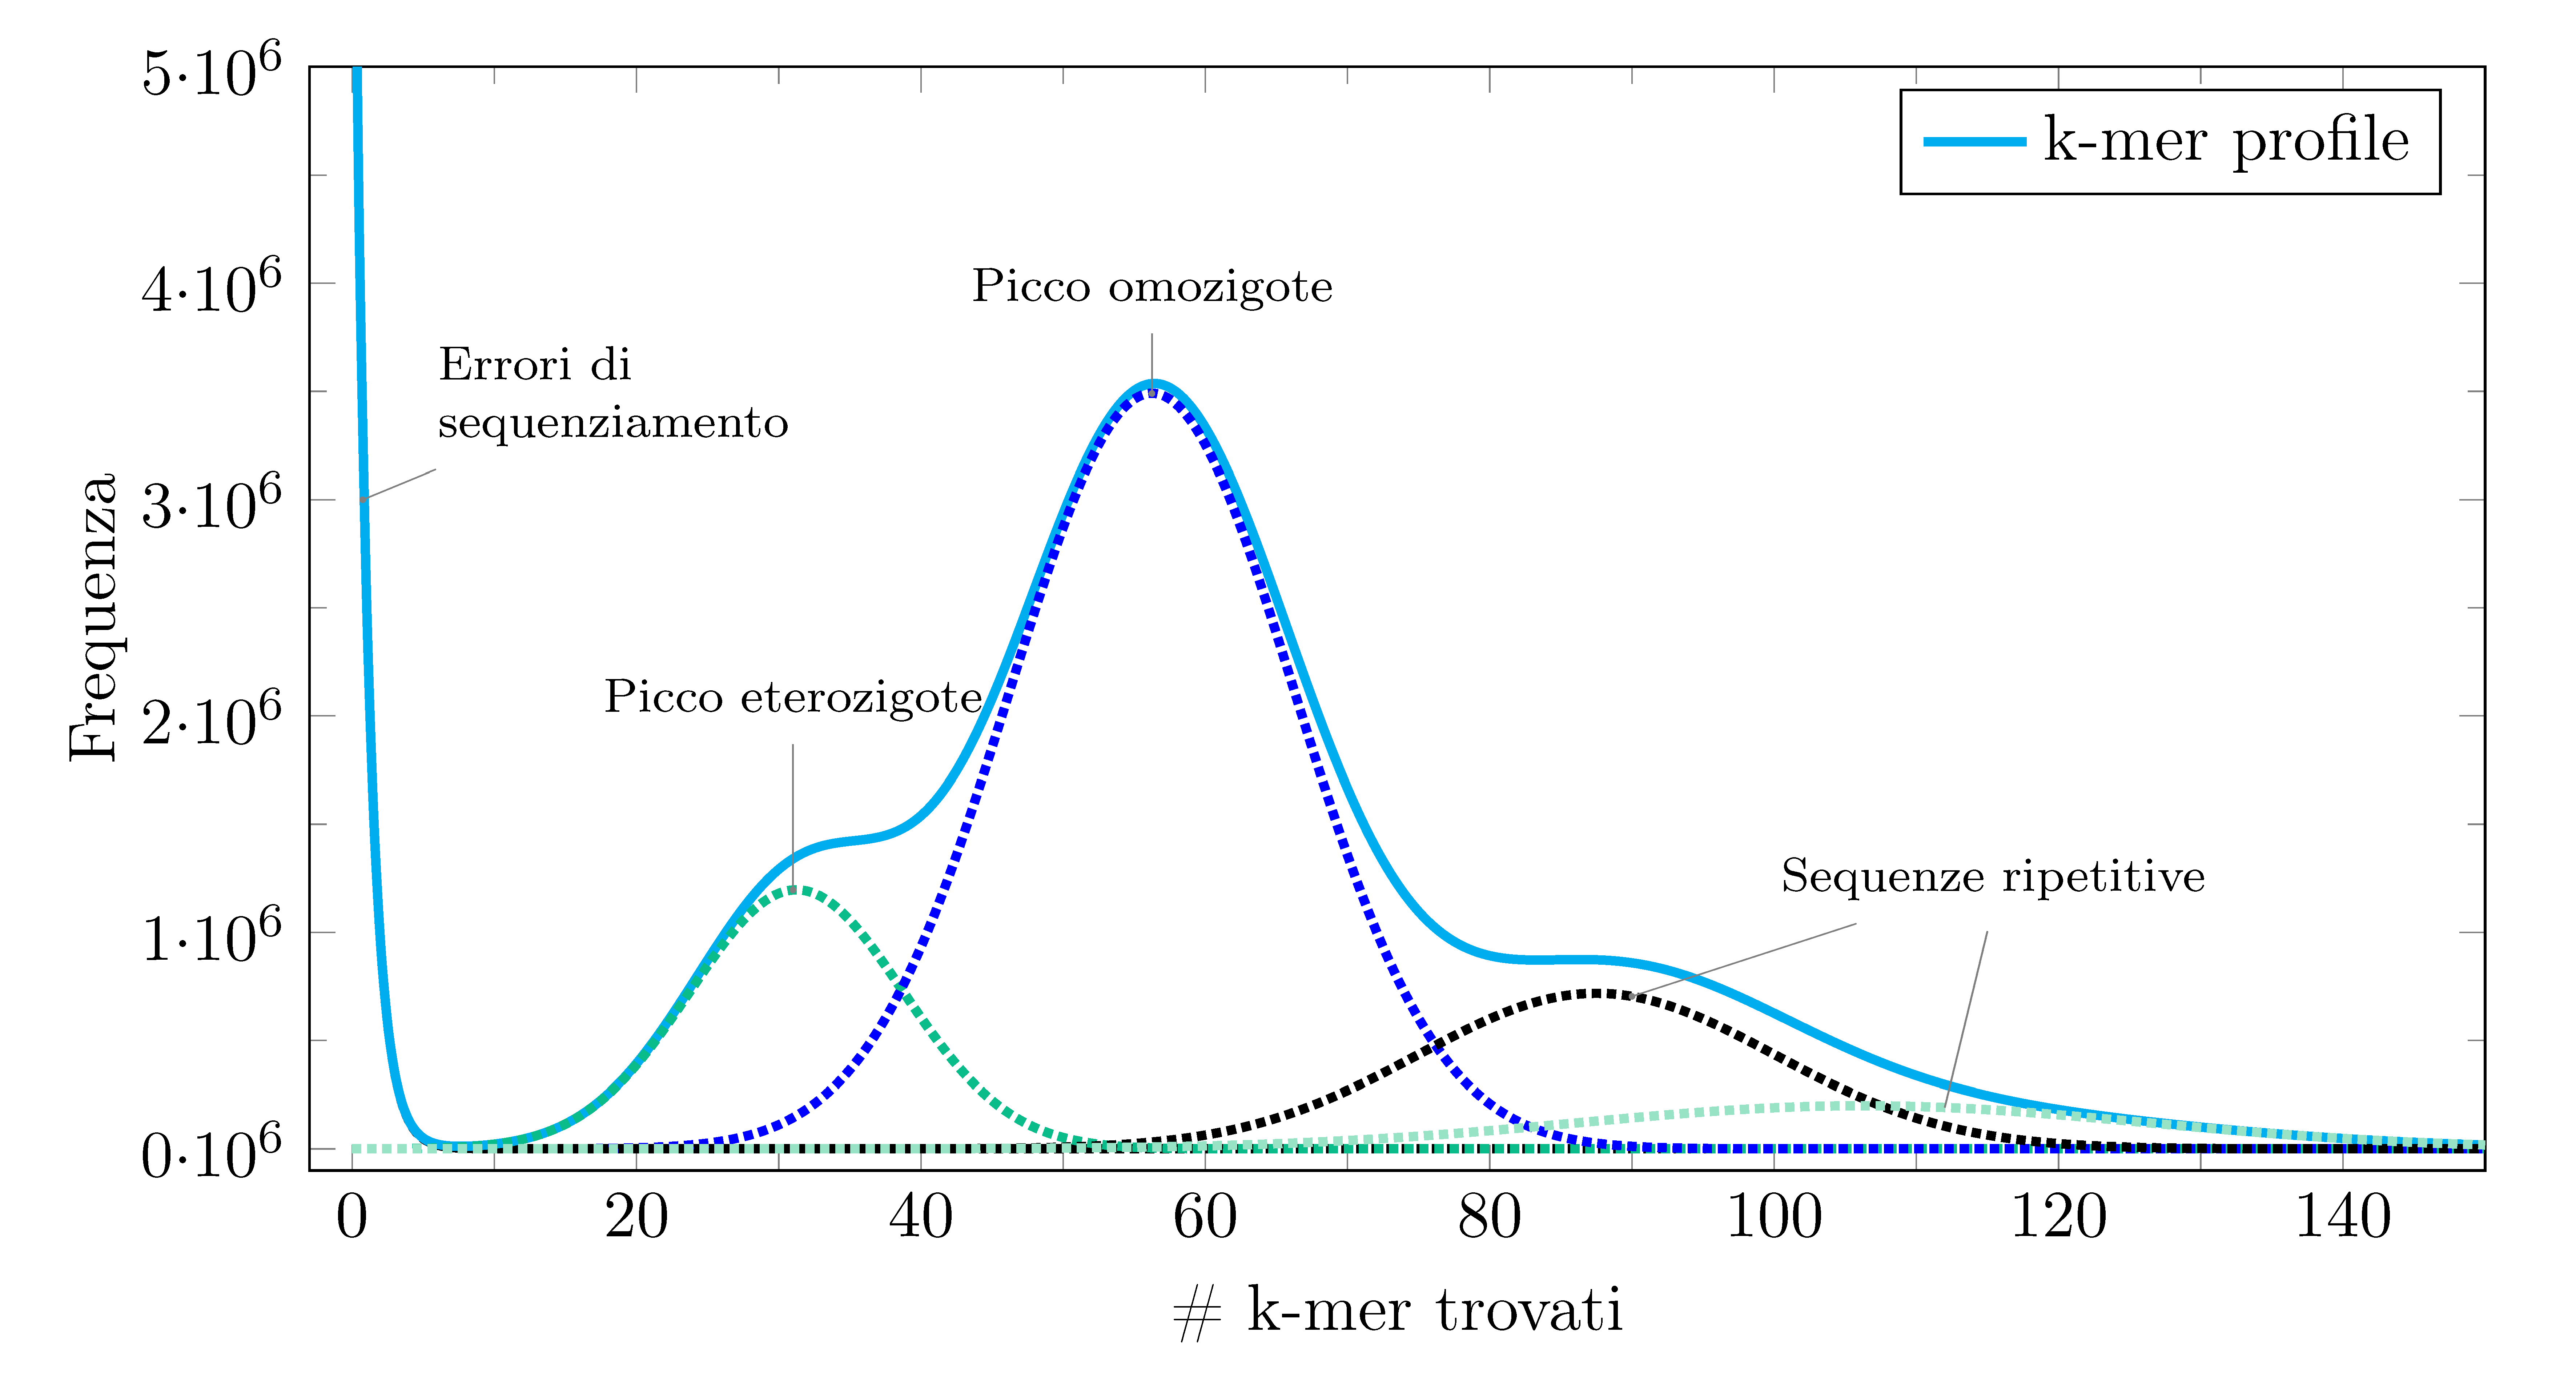
\includegraphics[width=0.8\textwidth]{capitoli/introduzione/profilecomp.png}
		\caption{Composizione di un k-mer profile.}
		\label{fig:profilecomp}
	\end{figure}
	
	Ipotizzando che il genoma sia ideale, omozigote e senza ripetizioni, e che le letture siano state fatte senza errori con una certa copertura, il grafico del k-mer profile sarà una \gls{dp} centrata sulla copertura media disponibile \cite{li2003estimating}.
	
	In casi reali invece, il genoma sarà eterozigote con una certa percentuale di eterozigosi e saranno presenti errori di sequenziamento; il k-mer profile presenterà tre picchi principali~\cite{sun2017findGSE}.
	Il primo picco del grafico corrisponde ai k-mer derivati da errori di sequenziamento, che accadono spesso ma che hanno bassa frequenza perché presentano poche occorrenze nelle letture di input; il secondo invece, rappresenta i k-mer eterozigoti e il terzo quelli omozigoti, presenti quindi su uno o entrambi gli alleli del set di cromosomi. I k-mer eterozigoti devono essere trattati più attentamente, perché possono risultare simili a quelli del primo picco, derivanti da errori di sequenziamento~\cite{sohn2016present}.	
	
	La lunga coda della distribuzione rappresenta invece le sequenze ripetitive, che occorrono con alta frequenza e sono presenti in un elevato numero di \gls{locus}. Eventuali ripetizioni aggiungono al grafico ulteriori picchi, mentre errori nelle letture aumentano la varianza e producono distorsioni nel grafico.
	
	La figura~\vref{fig:kmerprofile} tratta da \cite{vurture2017genomescope} mostra come all'aumentare del \gls{rate_eterozigosity} la quantità di k-mer eterozigoti del secondo picco diventi dominante rispetto ai k-mer omozigoti del terzo picco, che invece diminuiscono.
	
	\begin{figure}
		\centering
		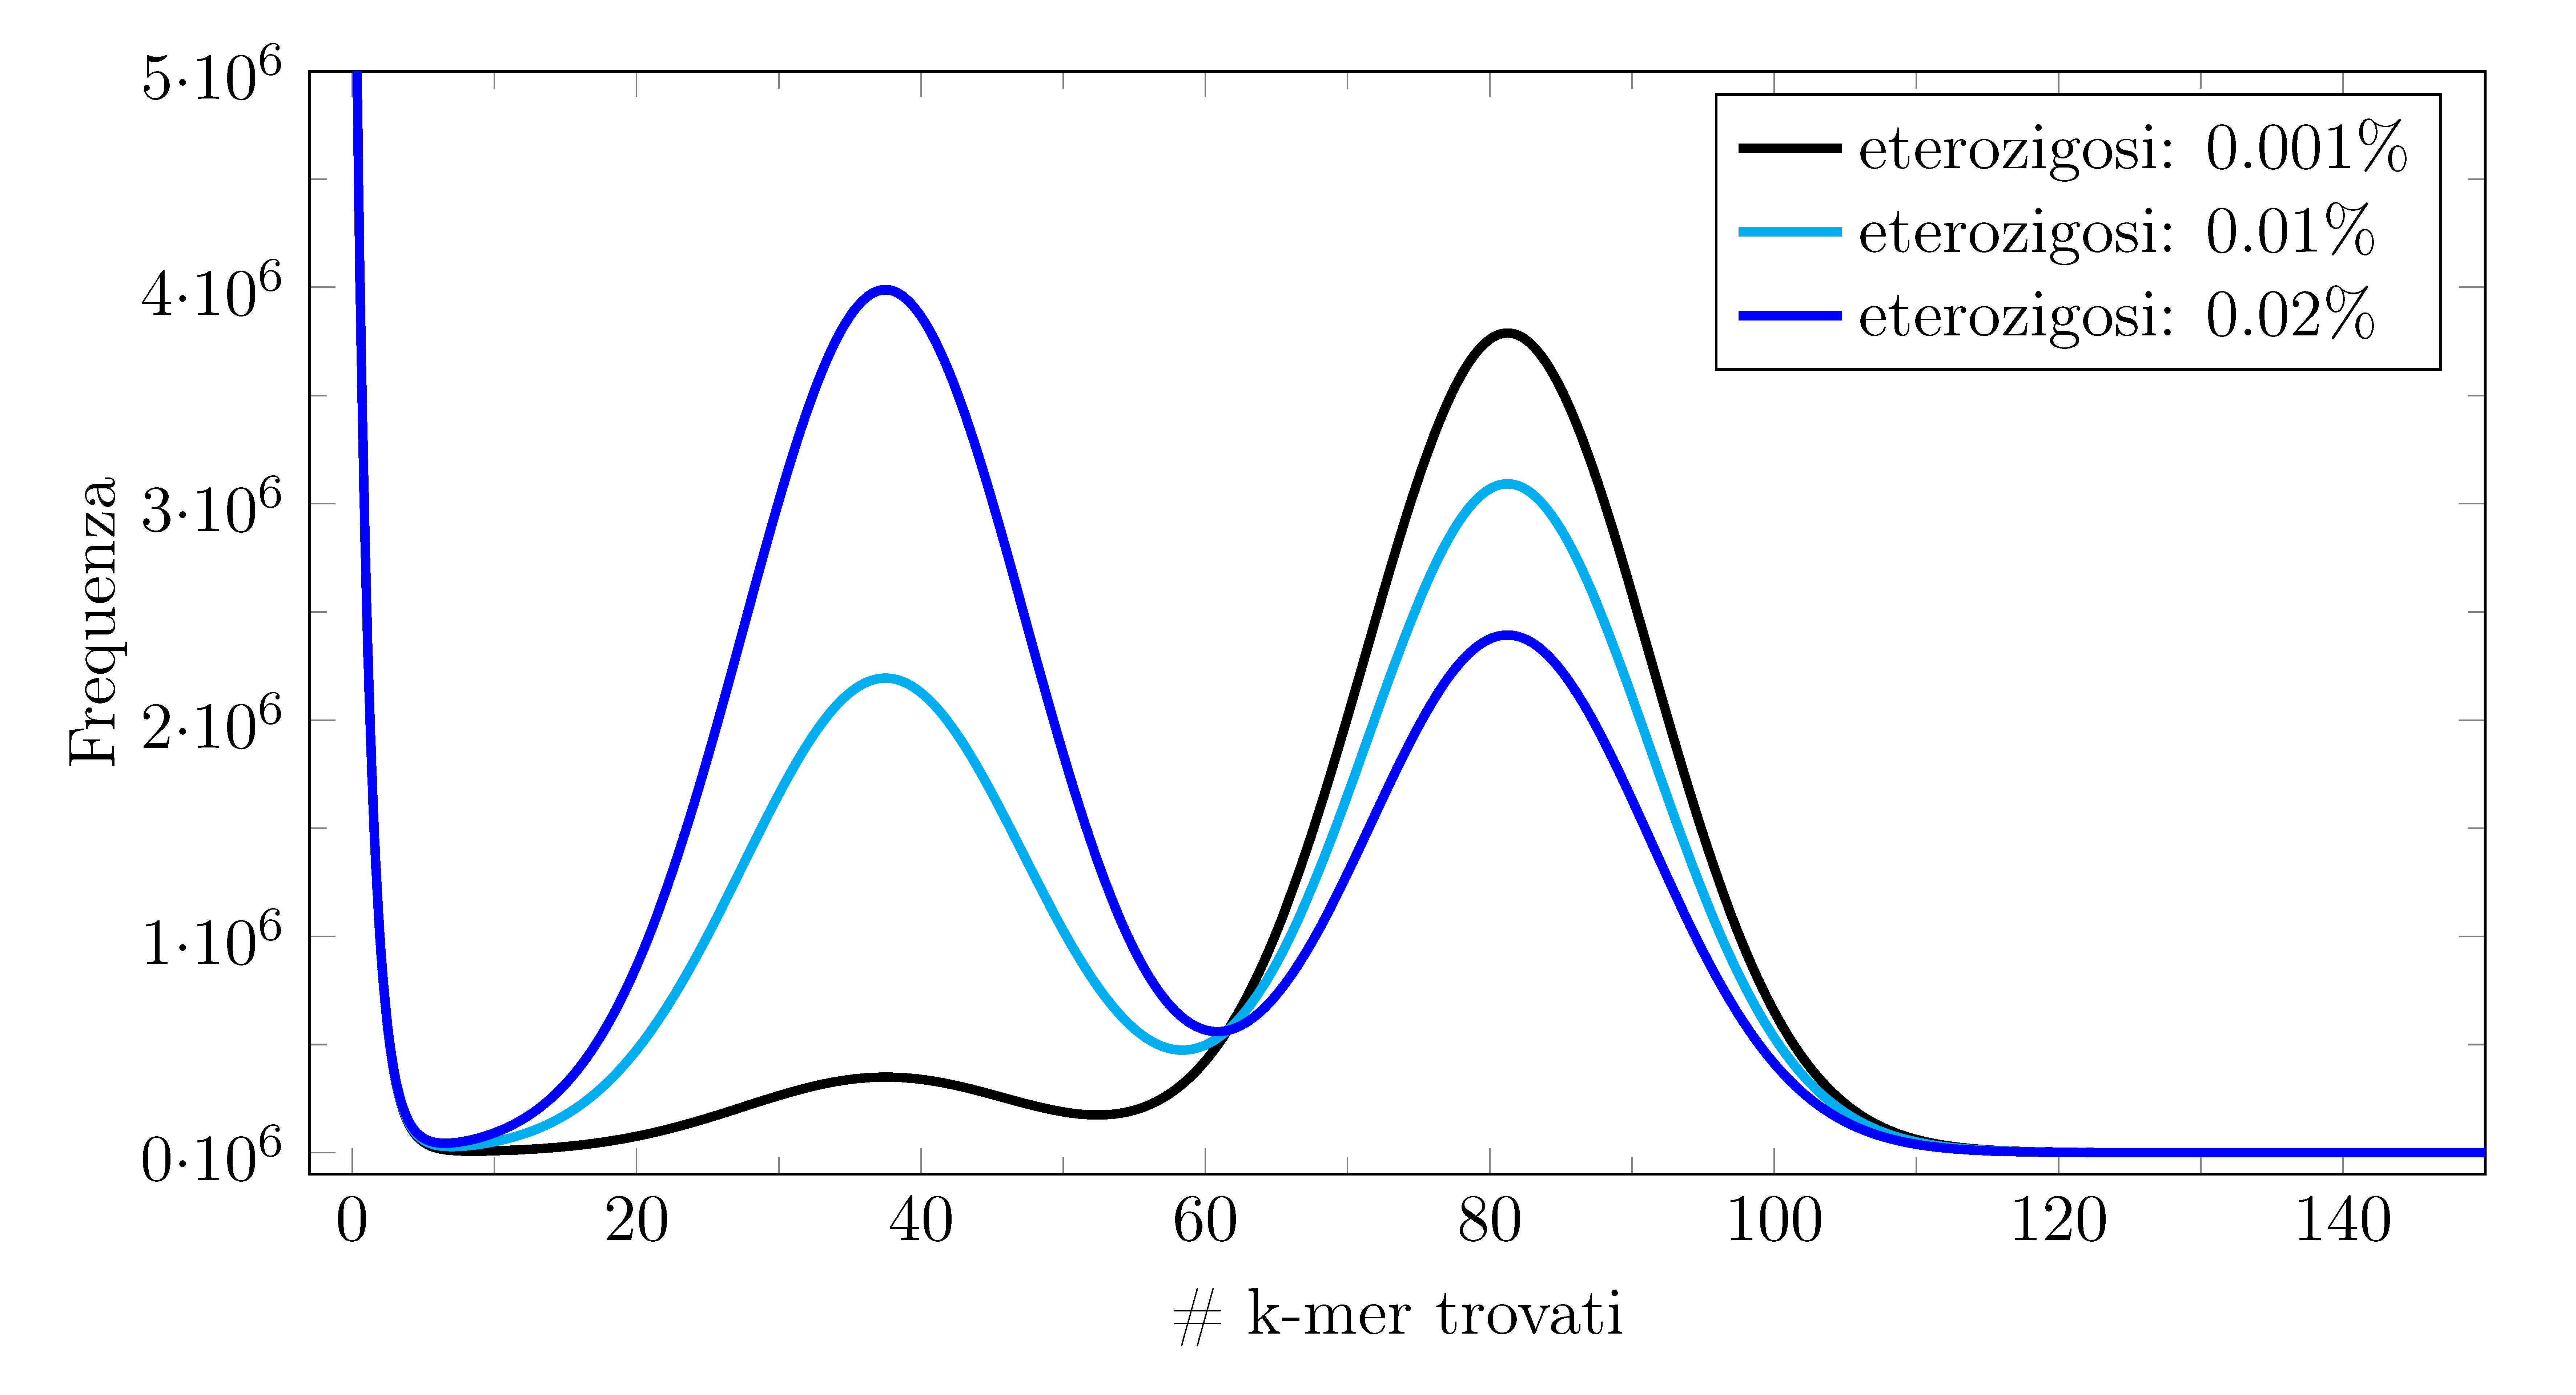
\includegraphics[width=0.8\textwidth]{capitoli/introduzione/kmerprofile.png}
		\caption{Variazione del grafico del k-mer profile al variare dell'eterozigosi.}
		\label{fig:kmerprofile}
	\end{figure}

\end{document}